\documentclass[journal,onecolumn]{IEEEtran}
\usepackage[utf8]{inputenc}
%\usepackage{hyperref}
\usepackage[sort,compress]{cite}
\usepackage{algorithmic}
\usepackage[ruled,linesnumbered,lined]{algorithm2e}
\usepackage{booktabs}

\usepackage{amsfonts}%Usando fontes para conjuntos numéricos

%\usepackage{titlesec}
\usepackage{color,colortbl,multirow}
\usepackage{xy}
\usepackage{graphicx,url, amsmath, color}
\usepackage{graphicx}
\usepackage{titling}

\newcommand{\subtitle}[1]{%
  \posttitle{%
    \par\end{center}
    \begin{center}\large#1\end{center}
    \vskip0.5em}%
}
\title{Relatório de projeto de segunda VA}
\subtitle{Réplica do trabalho:Simple face-detection algorithm based on minimum facial features}
\author{		Ismael Cesar da Silva Araujo
  				Departamento de computação \\
				  Ciência da computação\\
		Universidade Federal Rural de Pernambuco (UFRPE)\\
			ismael.cesar@ufrpe.br}
\date{}
\begin{document}
\maketitle

\section{Introdução}

\section{Conceitos Básicos}
	\label{sec:conceitosBasicos}
	O algoritmo em \cite{chen2007simple} pode ser dividido em três passos diferentes. 
	Detecção de Pele e cabelo, onde são computados os valores que representam os intervalos de cores de pele e cabelo para a binarização. 
	Quantização de pele e cabelo, onde uma vez binarizadas as detecções são aplicadas operações morfológicas, são computatos os componentes conexos e suas características e aplica-se os filtros de tamanho.
	Ao final, é feita a união das características, procurando intesecções entre retângulos que contém componentes conexos de cabelo e retângulos que contém componente conexos de pele.
	Como as etapas de detecção de pele e de cabelo são feitas de modo ligeiramente diferente, a explanação do funcionamento de ambas foi colocada em duas seções diferentes.
	Porém as etapas de quantização e união de características ocorre de maneira similar, tanto para deteção de cabelo quanto para detecção de pele.
	
	\subsection{Detecção de pele}
	\label{subsec:deteccaoPele}
	O modelo de cor normalizado, trata-se de um tipo de normalização feita por pixel. 
	Considerando uma com canais RGB (Sigla em inglês para Vermelho, Verde e Azul), 
	A normalização da imagem segundo o modelo de cor normalizada calcularia pra cada pixel o valor contido no canal dividido pela soma de todos os valores dos canais no pixel avaliado~\cite{chen2007simple,loesdau2017chromatic}. 
	Seja $\varepsilon$ uma constante da ordem de $10^{-8}$ somada a o denominador para se evitar divisão por zero\eqref{eq:nomalizedColorModel}.	
	\begin{equation}
		\begin{split}
			r  = \frac{R}{R+G+B+\varepsilon} \\\\
			g  = \frac{G}{R+G+B+\varepsilon} \\\\
			b  = \frac{B}{R+G+B+\varepsilon}
			\label{eq:nomalizedColorModel}
		\end{split}
	\end{equation}		
	A normalização das cores da imagem possibilitam a diminuição da sensibilidade do algorítmo de detecção em relação as variações de cores e illuminação.
	Normalizados os intervalos de valores do pixel, é necessário definir funções que avaliam os tons de vermelho  que foram normalizados.
	Tais funções são utilizadas para a definição dos limites superiores e inferiores do intervalo de tons de pele em relação ao canal $r$~\cite{soriano2000using,chen2007simple}.
	\begin{equation}
		\begin{split}
			F_1(r)  = -1.367r^2 + 1.0743r + 0.2 \\
			F_2(r)  = -0.776r^2 + 0.5601r + 0.18
		\end{split}
	\end{equation}
	
	Para o aprimoramento da detecção de pele necessário definir funções para avaliação de tons e branco, em conjunto com valores de matiz ou \textit{Hue} do píxel.
	A avaliação dos tons de branco é feita segundo os valores dos canais $r$ e $g$ do píxel. 
	De modo que o píxel é considerado com algum tom de branco quando $r=0.33$ e $g=0.33$~\cite{chen2007simple}.
	Onde a diferença dos valores dos canais $r$,$g$ e $0.33$ é elevada ao quadrado para para que a mesma só retorne o valor absoluto caso $r$ e $g$ possuam valores menores que $0.33$.
	
	\begin{equation}
		White(r,g) = (r - 0.33)^2 + (g - 0.33)^2 
		\label{eq:whiteValue}
	\end{equation}
	
	Para se constar se o píxel em questão tem algum tom de branco, verifica-se o resultado da comparação entre $White(r,g) > 0.001$.
	Para melhorar o desempenho da detecção de pele é necessário computar a relação entre o modelo de cor HSI (Hue Saturation and Itensity) com o modelo RGB.
	Onde \textit{Hue} descreve a cor que está sendo utilizada, o valor está no intervalo em $[0,360]$ o qual representa o ângulo no circulo unitário.
	\textit{Saturation} representa o nível de puresa da cor, e \textit{Intensity} trata-se de um valor acromático , que representa a itesidade da cor.
	Tanto o valor de \textit{Saturation} quanto o de \textit{Itensity} estão no intervalo de $[0,1]$.
	A figura a seguir ilustra o espaço de cores do modelo HSI. 

		\begin{figure}[htb]
		\begin{center}		
			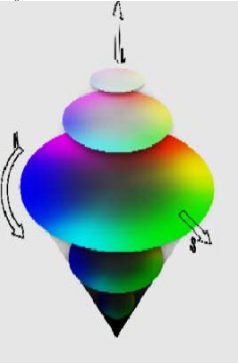
\includegraphics[scale=0.3]{espaco_hsi.png}
			\caption{Espaço de cores do modelo de cores HSI. fonte:\cite{ibraheem2012understanding} }
			\label{fig:espacoCoresHSI}
		\end{center}
		\end{figure}
	
	Para o algoritmo de detecção de só é necessário computar os valores relativos a \textit{Hue} e \textit{Intensity}.
	O valor de \textit{Hue} é atribuido segundo os valores B e G do esquema RGB. 
	Porém, antes de se computar o valor de \textit{Hue} é necessário computar o ângulo a qual o valor de RGB do pixel correspondem no espaço de cores do esquema HSI Fig.~\ref{fig:espacoCoresHSI}.
	As equações para computar os valores de ângulo, \textit{Hue} e \textit{Intensity} respectivamente encontra-se a seguir:
	
	\begin{equation}
		\theta (R,G,B) = cos^{-1}\left( \frac{0.5((R-G)+(R-B))}{\sqrt{(R-G)^2 +(R-B)(G-R) }} \right)
		\label{eq:angle}	
	\end{equation}
	\begin{equation}
	Hue(B,G,\theta) = 	\begin{cases}
						\theta,  \text{if } B \leq G \\
						360^\circ - \theta,  \text{if } B > G
						\end{cases}
	\label{eq:hue}
	\end{equation}
	\begin{equation}
	I(R,G,B) = 	\frac{1}{3} (R+G+B)
	\label{eq:intensity}
	\end{equation}

	Para se efetuar a detecção de pele numa imagem, faz-se uma binarização da imagem segundo os valores de computados segundo as equações mencionados.
	\begin{equation}
		SkinDetect = \begin{cases}
						1 , \text{ if }\left( g < F_1(r) \cap g > F_2(r) \cap White(r,g) > 0.001 \cap	
											(Hue(B,G,\theta) > 240^\circ \cup Hue(B,G,\theta) \leq 20^\circ) \right) \\
						0 , \text{ otherwise }
						\end{cases}
	\label{eq:SkinDetect}
	\end{equation}
	
	\subsection{Detecção de Cabelo}
	
	Para a detecção de tons de cabelo também é efetuada uma binarização da imagem. 
	Ao se fazer a binarização da imagem utiliza apenas as equações \eqref{eq:angle}\eqref{eq:hue}\eqref{eq:intensity} como sub-rotinas.
	Outros valores de comparação considerados são as diferenças entre o valor B e os valores R e G.
	
	\begin{equation}
		HairDetect = \begin{cases}
						1 , \text{ if }\left( (I(R,G,B) < 80 \cap ((B-G)< 15 \cup (B-R) < 15))
										\cup (20^\circ < Hue(B,G,\theta) \leq 40^\circ ) \right) \\
						0 , \text{ otherwise }
						\end{cases}
	\label{eq:HairDetect}
	\end{equation}
	
	\subsection{Quantização de pele e cabelo}
	
	A etapa de quantização ocorrre de forma semelhante tanto para detecção de cabelo quanto para detecção de pele.
	Uma vez retornada as binarizações da imagens com as detecções de pele e cabelo, são aplicadas operações morfológicas nos retornos \textit{SkinDetetct} e \textit{HairDetect}.
 	Os elementos estruturantes tem de tamanho $5\times 5$.
	A morfologia é calculada para determinar se um pixel numa região pertence a um componente conexo de cabelo, pele, ou se o pixel varrido é apenas ruído de detecção.
	
	Em seguida, são computados os componentes conexos e as características dos mesmos de \textit{SkinDetetct} e \textit{HairDetect}.
	As características computadas são o centroide, a área do componente conexo e as posições $(x,y)$ dos pixels mais externos, tanto o mais mais acima e mais a esquerda, quanto o mais abaixo mais a direita.
	Após a computação é feita uma filtragem de componentes conexos.
	Também chamado de filtro de tamanho, ou \textit{size filter}.
	O filtro de tamanho verifica a área de cada componente conexo e exclui o componente conexo cuja área é menor que um limiar qualquer $\lambda$.
	
	\subsection{União de características}	
	
	Para a união de características, faz-se o uso das posições $(x,y)$ computadas dos componentes conexos da detecção de cabelo e pele.
	Isso é feito devido a o fato das posições computadas das features representarem um retângulo que contém o componente conexo.
	Onde para cada componente conexo em $SkinDetect$ é verificado se há intersecção com algum componente conexo em $HairDetect$.
	Caso afirmativo, o algoritmo considera que achou uma face.
	Na figura \ref{fig:intesectRelations} são mostradas as relações de intesecção que são consideradas no algoritmo por simplicidade.
	\begin{figure}[htp]
	\begin{center}
		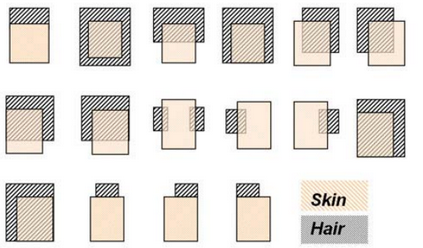
\includegraphics[scale=0.3]{intersections_skin_hair_components.png}
		\caption{Relações de intersecção entre retângulos que contém cabelo e pele, fonte:\cite{chen2007simple} }			\label{fig:intesectRelations}
	\end{center}
	\end{figure}
	
	\section{Metodologia}
	
	A réplica dos conceitos apresentados em \cite{chen2007simple} foram feitas utilizando python 3.6.
	Também foram utilizadas fuções das bibliotecas python OpenCV e numpy.
	As primitivas $F_1,F_2,\theta,White,Hue,I$  foram implementadas utilizando lambda expressões por simplicidade.
	Assim como na seção \ref{sec:conceitosBasicos} haverá uma explanação diferente nas etapas de deteção de cabelo e detecção de pele. 
	Isso acontecerá devido a fato de abordagens diferentes terem sido utilizadas tanto na réplica quanto na adaptação do código para que os resultados obtidos fossem parecidos ou até melhores.
	
	\subsection{Réplica: detecção de pele}
	
	Antes de se aplicar as primitivas de detecção de pele foi efetuada uma modificação do método de normalização.
	Primeiramente todos os valores contidos no array que represntava a imagem foram divididos por 255,chamado neste trabalho de nomalização geral.
	Somente em seguida é que foi aplicada uma normalização relativa a os valores das cores do pixel avaliado, segundo a Eq. \eqref{eq:nomalizedColorModel}.
	Isso foi feito pois, segundo observações experimentais, áreas pertencentes a um elemento de pele não estavam sendo detectadas como pelo algoritmo.
	
	Aplicando somente a normalização relativa pixel a pixel, o intervalo de valores de regiões com tonalidades de cor de pele não se encontravam nos limites das primitivas da subseção \ref{subsec:deteccaoPele}.
	Outra modificação aplicada foi a comparação da equação \eqref{eq:SkinDetect} em relação a o valor de $Hue$.
	O ângulo é retornado valores em radianos não em graus.
	Sendo o maior e o menor ângulo da comparação na equação $\frac{4}{3}\pi$ e $\frac{\pi}{4}$,  $240^\circ$ e $45^\circ$ respectivamente.
	Diferentemente do ângulo $20^\circ$ aprensentado na equação \eqref{eq:HairDetect}, foi empiricamente observado que o ângulo $45^\circ$ resultava em melhores detecções de regiões de pele.
	
	Sejam os valores $r,g,b$ os valores dos canais $RGB$ da imagem após a normalização geral seguida da normalização relativa pixel a pixel. 
	Os mesmos foram utilizados como entrada das primitivas $\theta (r,g,b)$ , $Hue(b,g,\theta)$ e $I(r,g,b)$.
	A comparação resultante das modificações da etapa de detecção de pele ficou como em Eq~\eqref{eq:newSkinDetect}.

		\begin{equation}
		SkinDetect = \begin{cases}
						1 , \text{ if }\left( g < F_1(r) \cap g > F_2(r) \cap White(r,g) > 0.001 \cap	
										(Hue(b,g,\theta) > \frac{4}{3}\pi \cup Hue(b,g,\theta) \leq \frac{\pi}{4} ) \right) \\
						0 , \text{ otherwise }
						\end{cases}
	\label{eq:newSkinDetect}
	\end{equation}
	
	\subsection{Réplica: detecção de cabelo}
	
	A mesma estratégia de aplicar uma normalização geral e normalização relativa pixel a pixel foram aplicadas na etapa de detecção de cabelo.
	Porém na comparação da equação \eqref{eq:HairDetect} foram efetuadas modificações, tanto na comparação dos valores de $Hue$ quanto na comparação dos valores de $I$ e nas diferenças entre os canais $B-G$ e $B-R$.
	Primeiramente, os algulos dos limites inferior e superior utilizados na comparação dos valores de $Hue$ foram $\frac{\pi}{4}$ e $\frac{\pi}{2}$, $45^\circ$ e $90^\circ$ respectivamente.
	Diferentemente dos $20^\circ $ e $40^\circ$ mostrados na equação \eqref{eq:HairDetect}, foi empiricamente observado que os ângulos $45^\circ$ e $90^\circ$ resultavam e detecções melhores de regiões de cabelo.
	
	Assim como na réplica da detecção de pele, os valores normalizados $r,g,b$, também serviram de entrada das primitivas $Hue$, $I$ e $\theta$ utilizadas. 
	Os mesmos também foram utilizados na computação das diferenças entre o canal azul e os canais verde e vermelho.
	Dado o fato de que os valores estão normalizados, os valores comparados com aqueles que as primitivas e as diferenças computam foram divididos por $255$.
	Empiricamente foi observado que esta ação resultava em boas detecções de cabelo.
	A comparação resultante das alterações ficou como em Eq~\eqref{eq:newHairDetect}
	
	\begin{equation}
		HairDetect = \begin{cases}
					1 , \text{ if }\left( (I(r,g,b) < 0.313 \cap ((b-g)< 0.0588 \cup (b-r) < 0.0588))
									\cup (\frac{\pi}{4} < Hue(b,g,\theta) \leq \frac{\pi}{2} ) \right) \\
					0 , \text{ otherwise }
					\end{cases}	
	\label{eq:newHaitDetect}
	\end{equation}
	
	\subsection{Réplica: quantização de cabelo e pele}
	
	Uma vez obtidas as binarizações das imagens segundo a detecções de pele cabelo, faz-se uma computação de componentes conexos junto com suas features básicas, a partir da chadada do procedimento $connectedComponentsWithStats(binaryImage)$, onde $binaryImage$ é a imagem binarizada.
	
	A única modificação quanto a etapa de quantização tanto de pele quanto de cabelo foi feita quanto a aplicação das operações morfológicas das imagens binarizadas.
	Para operação morfológica na binarização da detecção de pele o tamanho do elemento estruturante foi modificado de $5 \times 5$ para $10 \times 10$.
	E foram efeutadas duas operações de erosão seguidas de duas operações de dilatação. 
	Foi empiricamente observado que tais sequências de operações resulta numa melhor remoção de ruído de detecção de pele.

	Para binarização resultante da detecção de cabelo, o elemento estrutuarante foi modificado de $5 \times 5$ para $3 \times 3$.
	 Foi aplicada apenas uma operação de abertura.
	 Semelhantemente, foi empiricamente observado que tais modificações resultavam numa melhor remoção do ruído de detecção de cabelo.
	 
	 \subsection{Réplica: união de características}
	 
	Uma vez computadas as características dos componentes conexos da quantização de cabelo e face passa-se para a etapa de união de características.
	O algoritmo proposto em \cite{chen2007simple} considera que caso não haja intersecção então não foi detectada nenhuma face.
	Das características computadas a principal é o retângulo que contém o componente conexo que representa uma detecção de cabelo ou de face.
	
	Na réplica, ao invés de simplesmente verificar a existência de intersecção entre retângulos a partir dos pontos.quantização
	Foi efetuado o cálculo da área da intersecção entre os retângulos que contém os componentes conexos da detecção de cabelo e detecção de pele.
	Desse modo é possível distinguir entre intesecções maiores entre retângulos, e remover intersecções resultantes de detecções espúrias resultantes de ruídos que conseguiram passar pela etapa de quantização.
	O cálculo das posições $(x,y)$ dos vértices do retângulo de intersecção foi feito segundo Eq.\eqref{eq:intersectionPositions}.
	 
	 \begin{equation}
	 	\begin{cases}
	 	x_1 = max(hairL.x,skinL.x) \\
	 	y_1 = max(hairL.y,skinL.y) \\
	 	
	 	x_2 = min(hairR.x,skinR.x) \\
	 	y_2 = min(hairR.y,skinR.y) 
	 	\end{cases}
	 	\label{eq:intersectionPositions}
	 \end{equation}
	 
	Onde $hairL$ e $skinL$ são os vértices superiores mais a esquerda dos retângulos que contém os componentes conexos de detecção de cabelo e pele respectivamente.
	E $hairR$ e $skinR$ os vértices inferiores mais a direita.
	
	\section{Resultados}
	O algoritmo proposto é extremamente dependete das cores da imagem. 
	Apesar do uso das cores como característica de deteção de detecção ser simples de utilizar, seu pode resultar  em detecções espúrias.
	Principalmente em regiões que não pertencem a pele ou cabelo do indivíduo, mas são detectadas como tal pois o possuem uma tonalidade de cor parecida com que consta no intervalo de cor das primitivas implementadas.
%Resultados Bons
\begin{figure}[htb]
\resizebox{.9 \textwidth}{!}{
\begin{tabular}{cccccc}

	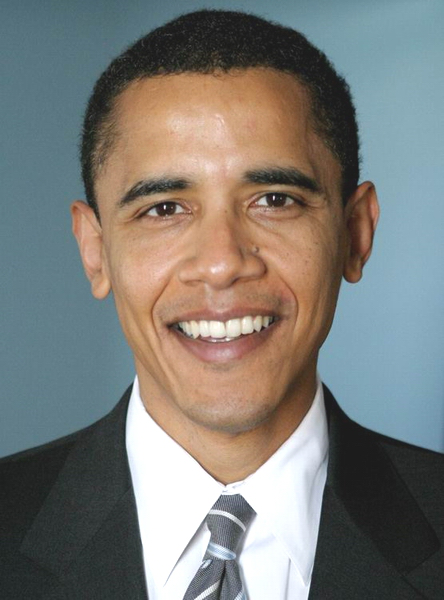
\includegraphics[scale=0.3]{images/Original.png}
  &

	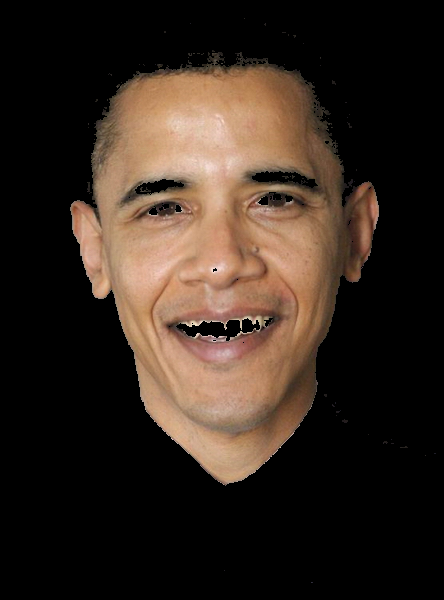
\includegraphics[scale=0.3]{images/skinDetect.png}

&

	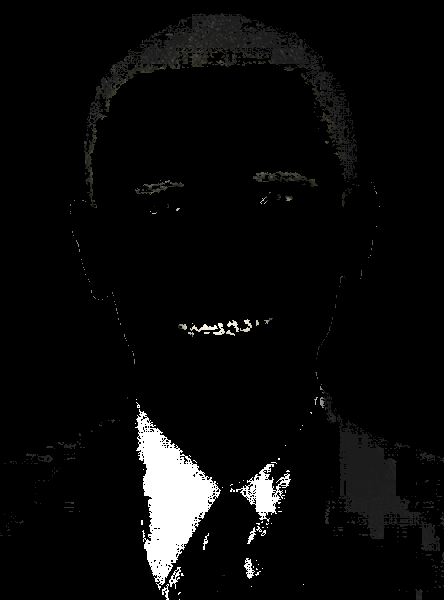
\includegraphics[scale=0.3]{images/hairDetect.png}

&

	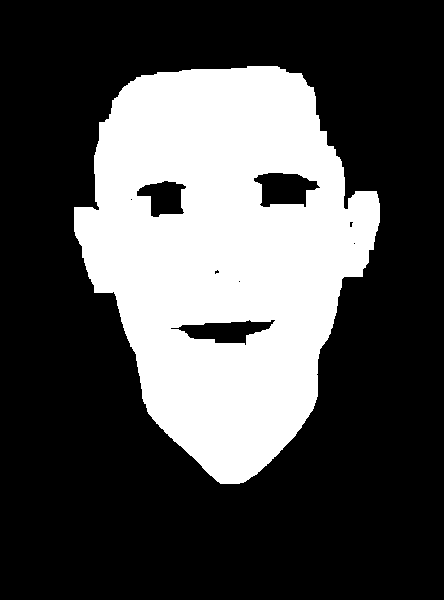
\includegraphics[scale=0.3]{images/skinQuantization.png}

&

	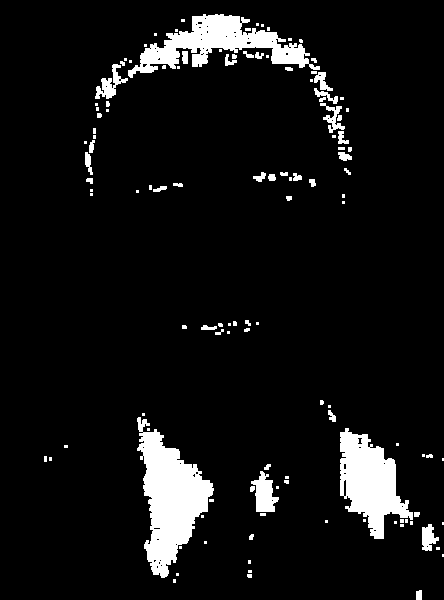
\includegraphics[scale=0.3]{images/hairQuantization.png}

&

	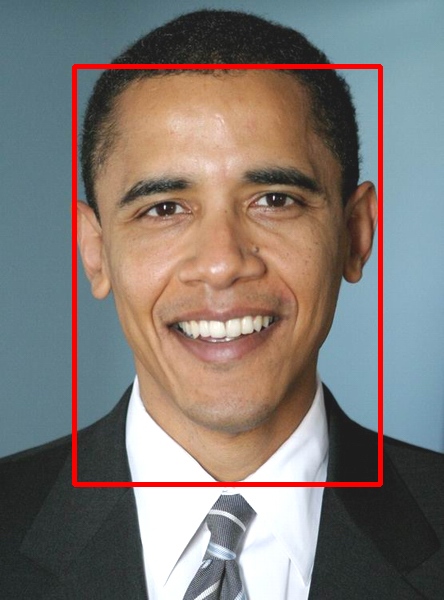
\includegraphics[scale=0.3]{images/Detection.png}
\\
Original & Skin Detection & Hair Detection & Skin Quantization & Hair Quantization & Detection\\
\end{tabular}
}	
\caption{Resultados de deteção de pele e cabelos segundo as etapas descritas na seção de metodologia}
\label{fig:goodDetection}
\end{figure}  

	Na figura \ref{fig:badDetection} é possível notar detecções espúrias relacionadas a dependência de cores do algorítmo.
	Apesar do indivíduo detectado não ter cabelo, o algorítmo detectou a face do mesmo devido a intersecção de componentes de cabelo ao fundo da imagem e componentes de face que estão próximos.
%Resultados spurios
\begin{figure}[h]
\resizebox{.9 \textwidth}{!}{
\begin{tabular}{cccccc}

	
\includegraphics[scale=0.3]{images/OriginalSpurious.png}
  &

	
\includegraphics[scale=0.3]{images/skinDetectSpurious.png}

&

	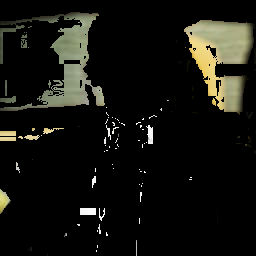
\includegraphics[scale=0.3]{images/hairDetectSpurious.png}

&

	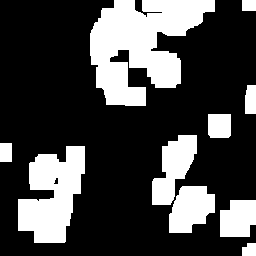
\includegraphics[scale=0.3]{images/skinQuantizationSpurious.png}

&

	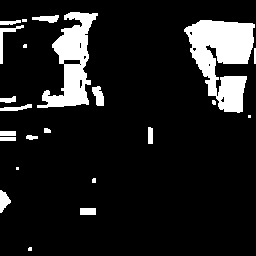
\includegraphics[scale=0.3]{images/hairQuantizationSpurious.png}

&

	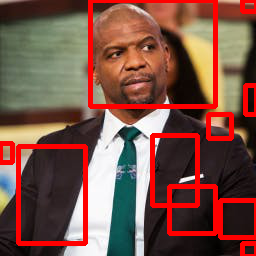
\includegraphics[scale=0.3]{images/DetectionSpurious.png}
\\
Original & Skin Detection & Hair Detection & Skin Quantization & Hair Quantization & Detection\\
\end{tabular}
}	
\caption{Resultados espúrios de deteção de pele e cabelos segundo as etapas descritas na seção de metodologia}
\label{fig:badDetection}
\end{figure}  
	
	Algo similar acontece quando se trata de regiões que são identificadas como face simplesmentes por ter uma tonalidade de cor cujo valor se encontra no intervalo das primitivas implementadas.	
	Na figura \ref{fig:badMultifaceDetection} é possível observar que a detecção de uma região muito grande como se fosse um rosto.
	Também é possível notar a existência de detecções que não pertencem a um rosto.
	Mas que foram detectadas como tal devido a computação de intesecções de regiões detectadas como cabelo estavam muito próximas das mesmas.
	%Resultados multiplos
\begin{figure}[htb]
\resizebox{1 \textwidth}{!}{
\begin{tabular}{cc}

	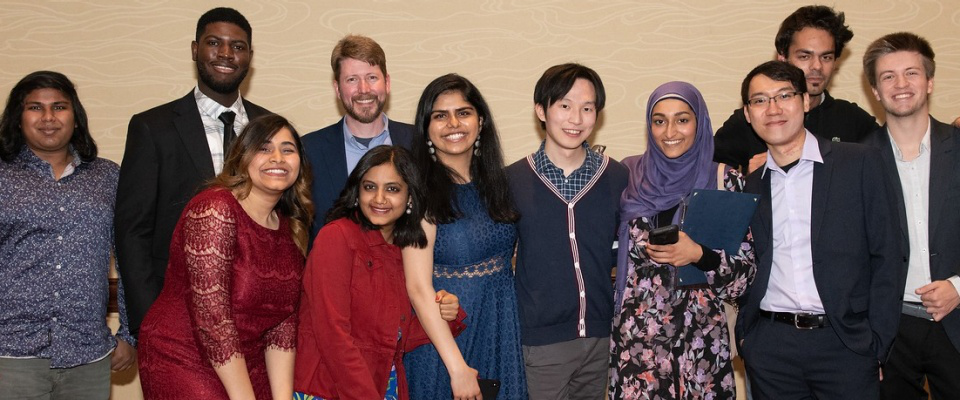
\includegraphics[scale=0.3]{images/OriginalSpurious2.png}
  &

	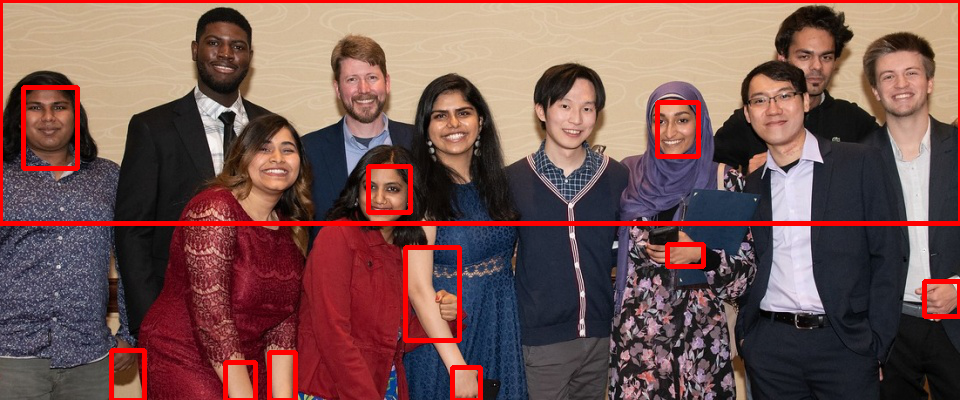
\includegraphics[scale=0.3]{images/DetectionSpurious2.png}
\\
Original &  Detection\\
\end{tabular}
}	
\caption{Resultados espúrios de detecção multiface}
\label{fig:badMultifaceDetection}
\end{figure} 


	\section{Trabalhos Futuros}
%Deixar para o final
	O algoritmo proposto em \cite{chen2007simple} tem como objetivo detectar faces de acordo com o mínimo possível de características.
	Porém por ser altamente dependente das cores presentes na imagem, mesmo pode acabar resultando em outliers muito distantes do que seria uma detecção de face ideal.
	Porém tal algoritmo pode ser como uma heurística para melhorar algoritmos de aprendizagem de máquina que efetuam detecção de face.
	Os algoritmos mais simples geralmente efetuam uma varredura completa na imagem para poder propagar os mapas de características ao longo das camadas.
	Um possível trabalho futuro seria investigar se utilização deste algoritmo para definir regiões de interesse  deixaria outros algoritmos de aprendizagem de máquina para detecção de face mais eficientes e precisos.
	
\bibliographystyle{IEEEtranS}
\bibliography{bibliography}
\end{document}

